\begin{center}
	\section{\textit{M\'etodo de elementos discretos} - DEM}
\end{center}

\noindent
\justify

El m\'etodo de elementos discretos (DEM) es un m\'etodo que modela fuerzas interpart\'icula basadas en par\'ametros de elasticidad y la superposici\'on de part\'iculas no deformadas, que se entiende como la cantidad de deformaci\'on necesaria para que puedan, f\'isicamente, ocupar el espacio en su actual configuraci\'on. Requiere de seis grados de libertad en cuerpos r\'igidos: tres en dos dimensiones y seis en tres dimensiones.

\begin{figure}[h!]
	\centering
	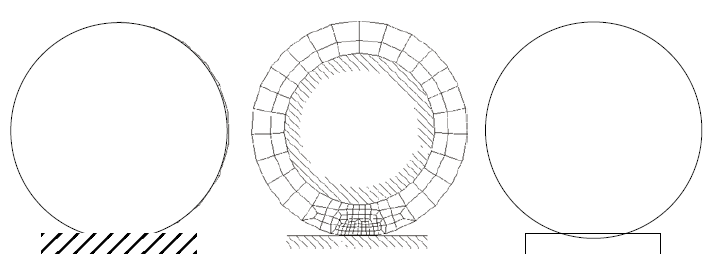
\includegraphics[width=\textwidth]{Images/DEM.PNG}
	\label{dem}
	\caption{Comparaci\'on entre metodolog\'ias de an\'alisis de part\'iculas para una esfera suave deformada en un plano: situaci\'on f\'isica real (izquierda), modelo analizado con el m\'etodo de elementos finitos (centro) y modelo con el m\'etodo de elementos discretos (derecha)}
\end{figure}

\noindent
\justify

El principio de este m\'etodo es el de computar las fuerzas proporcionales a la superposici\'on geom\'etrica de las part\'iculas empleadas. Para part\'iculas esf\'ericas, o circulares, las fuerzas involucradas son de tipo central; a diferencia de otras configuraciones geom\'etricas, debido a que deben caracterizar las fuerzas en la forma `d\'ebil' y `fuerte'. 

\noindent
\justify

Una simulaci\'on que emplea este m\'etodo num\'erico, normalmente se rige bajo los siguientes pasos:

\begin{enumerate}
	\item Detecci\'on de colisi\'on entre part\'iculas.
	\item Creaci\'on de una nueva interacci\'on y determinaci\'on de diferentes propiedades, entre ellas la rigidez.
\end{enumerate}

\noindent
\justify

Para interacciones ya existentes:

\begin{enumerate}
	\item Evaluaci\'on de deformaci\'on.
	\item Computaci\'on del esfuerzo basada en la deformaci\'on.
	\item Aplicaci\'on de fuerzas en la interacci\'on entre part\'iculas.
\end{enumerate}

\subsection{Detecci\'on de una colici\'on}

\noindent
\justify

La detecci\'on \textit{exacta} de colisi\'on entre dos part\'iculas requiere de un alto costo computacional. Tomando una pareja de cuerpos $i$ y $j$ y su colisici\'on `exacta' (en el sentido de precisi\'on admisible por la implementaci\'on num\'erica) presentadas en los puntos $P_i$ y $P_j$ la detecci\'on procede en los siguientes dos puntos:

\begin{enumerate}
	\item Detecci\'on de colisi\'on r\'apida usando puntos aproximados $\widetilde{P}_i$ y $\widetilde{P}_j$; siendo estos preconstrucciones en el modo que caracter\'isticas individuales $P_i$ y $P_j$ satisfacen la siguiente condici\'on mostrada en la Ecuaci\'on \ref{cond}.
	\begin{equation}
		\forall x \in R^3 : x \in P_i \rightarrow x \in \widetilde{P}_i
		\label{cond}
	\end{equation}
	De igual manera para $P_j$. El predicado aproximaado se conoce como `volumen l\'imite', siguiendo lo siguiente:
	\begin{equation}
		\left(\widetilde{P}_i \cap \widetilde{P}_j \right) = {\O} \rightarrow \left( P_i \cap P_j \right) = {\O}
		\label{imposible}
	\end{equation}
	\item Al filtrar las colisiones imposibles mediante la Ecuaci\'on \ref{imposible}, algoritmos de detecci\'on de mayor costo computacional pueden ser impementados al filtrar falsas parejas de colisi\'on restantes, como se observa en la Figura \ref{colision}.
	\begin{equation}
		\left(\widetilde{P}_i \cap \widetilde{P}_j \right) \neq {\O} \wedge \left(P_i \cap P_j \right) = {\O}
	\end{equation}
\end{enumerate}

\begin{figure}[h!]
\centering
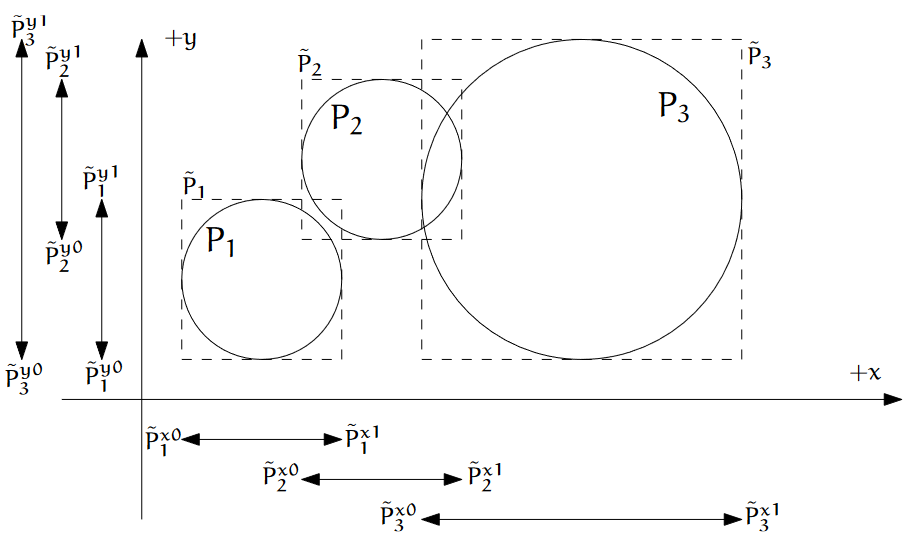
\includegraphics[width=0.85\textwidth]{Images/Colision.PNG}
\caption{Detecci\'on de colisi\'on entre part\'iculas.}
\label{colision}
\end{figure}